% Chapte 9
\chapter{Advertisement enhancement} % Main chapter title

\label{Chapter9} % For referencing the chapter elsewhere, use \ref{Chapter1} 

\section{Introduction}


\section{Introduction}


\section{Attraction attention}
\section{Motivation}
\section{Interaction}
\section{Design study}
\section{Data gathering}




\section{Findings and results}

\subsection{Attention Level measurements}


\begin{figure}[H]
    \centering
    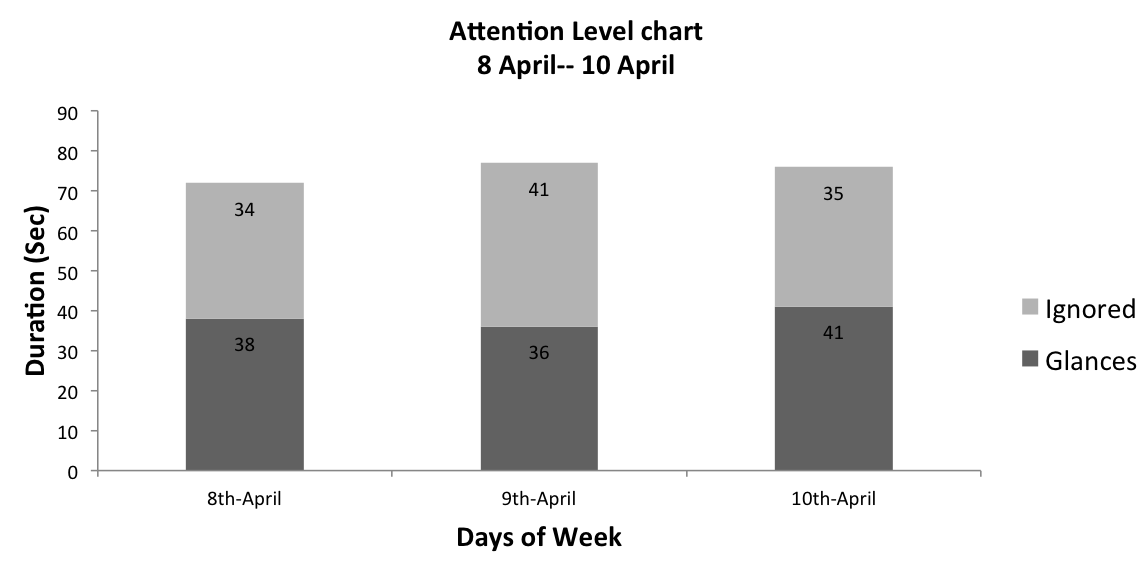
\includegraphics[width=110mm,height=55mm]{Figures/9/newbody_Inter_chart}%
    \caption{New body interactive attention level chart}%
    \label{fig:newbodyattentionlevelchart}%
\end{figure}



\begin{figure}[H]
    \centering
    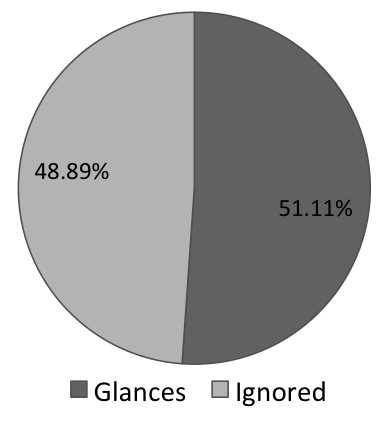
\includegraphics[width=110mm,height=55mm]{Figures/9/newbody_inter_percentage}
    \caption{Non-interactive Attention level percentage}%
    \label{fig:Nonattentionlevelpercentage}%
\end{figure}



\subsection{Engagement time}

\subsection{Passerby and engagement}



\begin{figure}[H]
    \centering
    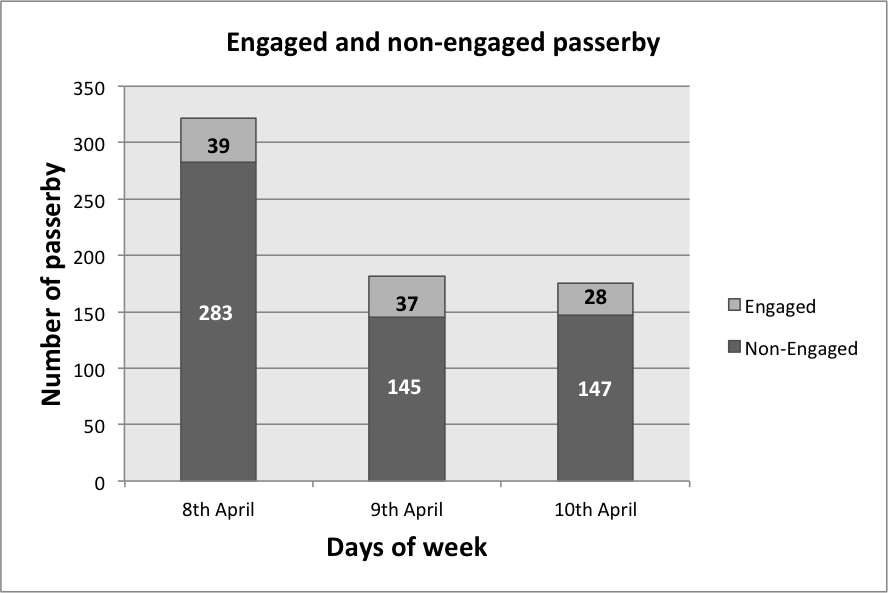
\includegraphics[width=110mm,height=60mm]{Figures/9/newbody_inter_engage_day}
    \caption{New body interaction Number of engaged passerby}%
    \label{fig:newbodyengagedandengagedby}%
\end{figure}

\begin{figure}[H]
    \centering
    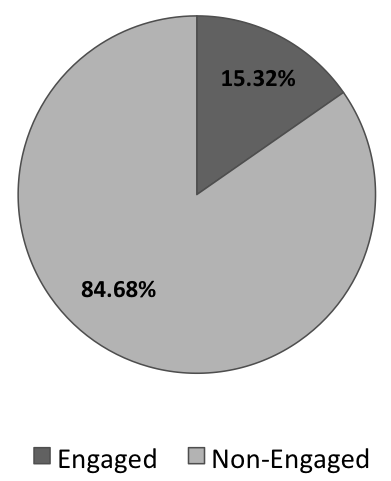
\includegraphics[width=110mm,height=60mm]{Figures/9/newbody_eng_percentage}
    \caption{New body Percentage of engaged and passerby}%
    \label{fig:newbodyengagedpasserbypercentage}%
\end{figure}




\subsection{Landing and Honeypot effects}

\begin{table}[H]
\caption{Landing and honeypot effects}
\label{tab:landingandhonypot}
\centering
\begin{tabular}{| l | c | c |}
\toprule
\tabhead{Days} & \tabhead{Landing effect} & \tabhead{Honeypot effect} \\
\midrule
\textbf{8th April}  & 3 &  3 \\
\textbf{9th April}  & 2 &  5 \\
\textbf{10th April}  & 1 &  2 \\
\bottomrule
\end{tabular}
\end{table}


\subsection{Note taking}

see Appendix Appendix \ref{AppendixE}.1

\subsection{Comparison with Body interaction}


\begin{enumerate}


\item Comparison of number of passerby
To be on safe side that the number of participants were statistically the same the bellow computation has be applied.
\begin{table}[H]
\caption{Number of people for three conditions}
\label{tab:newbodypasserbyofthreeweeks}
\centering
\begin{tabular}{| l | c | c | c |}
\toprule
\tabhead{Days} & \tabhead{Non-Interactive} & \tabhead{Body Interactive} & \tabhead{New-body Interactive} \\
\midrule
\textbf{Day 1}  & 212 & 259 &  322 \\
\midrule
\textbf{Day 2}  & 209 & 216 &  182 \\
\midrule
\textbf{Day 3}  & 208 & 122 &  175 \\
\midrule
\textbf{Total}  & 629 & 597 &  679 \\
\bottomrule
\end{tabular}
\end{table}


ANOVA test revealed that there is no significant different between the passers-by in each of the conditions (\emph{(F2,3)=0.1449, p >.05 (p=0.868)})



\item{Attention Level measurements}

\begin{table}[H]
\caption{Cross tabulation for each condition attention level }
\label{tab:newbodycrosstabulationweeks}
\centering
\begin{tabular}{| l | c | c | c |}
\toprule
\tabhead{Method} & \tabhead{Glanced (\%)} & \tabhead{Ignored} & \tabhead{Total } \\
\midrule
\textbf{Body Interactive}     	 & 96 (\%38.70)   &   152      &   248\\
\midrule
\textbf{New body Interactive }   & 108 (\%49.54)  &   110      &   218\\
\midrule
\textbf{Total }         		 & 204            &   262      &   466\\
\bottomrule
\end{tabular}
\end{table}

As can be seen the new body interactive advertisement has a higher percentage almost \%50 of the glances compared to the old body interactive advertisement.

To see if these are statistically significant different, the Chi-square test was applied on them.\\
${\chi}^2$\emph{(1, N=466)=5.5303, p < .05 (p=.01869)}





\item{Landing effects}


\begin{table}[H]
\caption{Cross tabulation for each condition Landing effect }
\label{tab:newbodylandingeffect}
\centering
\begin{tabular}{| l | c | c | c |}
\toprule
\tabhead{Method} & \tabhead{Non-Interactive} & \tabhead{Body Interactive} & \tabhead{New body Interactive } \\
\midrule
\textbf{Day 1}    & 2    &   2      &   1\\
\midrule
\textbf{Day 2 }   & 0    &   2      &   2\\
\midrule
\textbf{Day 3}    & 1    &   3      &   3\\
\bottomrule
\end{tabular}
\end{table}

ANOVA states that there is no significant different for these three days for all of the conditions.\\
(\emph{(F2,3)=1.857, p >.05 (p=0.236)})


\item{Honeypot effects}


\begin{table}[H]
\caption{Cross tabulation for each condition Honeypot effect }
\label{tab:newbodyhoneypoteffect}
\centering
\begin{tabular}{| l | c | c | c |}
\toprule
\tabhead{Method} & \tabhead{Non-Interactive} & \tabhead{Body Interactive} & \tabhead{New body Interactive } \\
\midrule
\textbf{Day 1}    & 2    &   2      &   3\\
\midrule
\textbf{Day 2 }   & 2    &   5      &   5\\
\midrule
\textbf{Day 3}    & 1    &   3      &   2\\
\bottomrule
\end{tabular}
\end{table}

ANOVA reveals that there is also no statistical difference between these conditions. \\
(\emph{(F2,3)=1.667, p >.05 (p=0.266)})




\item{Engagement time}

\item{Passerby and engagement}

\item{Note taking}


\end{enumerate}



\section{Discussions}
